\subsection{Теоритическая основа}

\qquad Frequency Shift Key - вид модуляции, при которой скачкообразно изменяется частота несущего сигнала в зависимости от значений символов информационной последовательности. Частотная модуляция весьма помехоустойчива, так как помехи искажают в основном амплитуду, а не частоту сигнала.

\begin{figure}[H]
	\begin{center}
		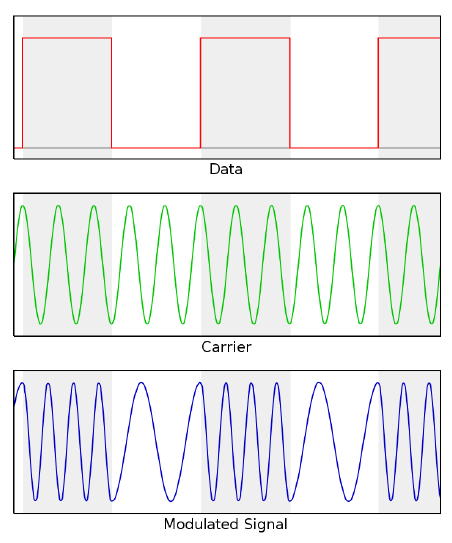
\includegraphics[scale=1]{fig/lab12/lab12_01.png}
		\caption{Пример FSK с двоичными данными}
	\end{center}
\end{figure}

\subsection{Схема в GNU Radio}    
    Для изучения этого процесса в GNU Radio необходимо построить следующую блок схему \ref{pic:fsk_scheme}:
    
    \begin{landscape}
    	\begin{figure}[H]
        		\centering
        		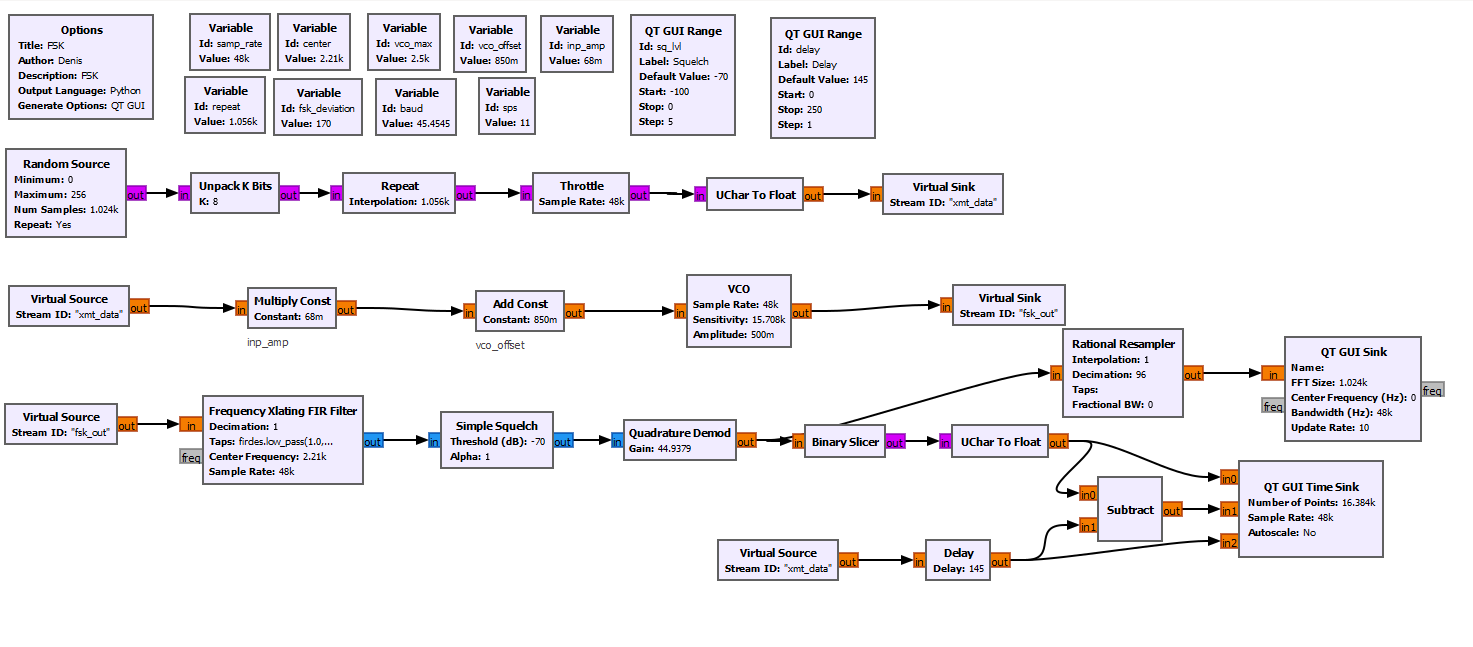
\includegraphics[width=25.5cm]{fig/lab12/lab12_02.png}
        		\caption{Схема FSK}
        		\label{pic:fsk_scheme} % название для ссылок внутри кода
    	\end{figure}
\end{landscape}

Описание используемых блоков:
\begin{itemize}
	\item Variable - блок адресующий в уникальной переменной. При помощи ID можно передавать информацию через другие блоки.
	\item QT GUI Range - графический интерфейс для изменения заднной переменной.
	\item Random Source - генератор случайных чисел.
	\item Unpack K bits - преобразуем байт с k релевантными битами в k выходных байтов по одному биту в каждом.
	\item Repeat - количество повторенний ввода, деуйствующее как коэффицент интерполяции.
	\item Throttle - дросселировать поток таким образом, чтобы средняя скорость не превышала удельную скорость.
	\item Uchar To Float - конвертация байта в Float.
	\item Virtual Sink - сохраняет поток в вектор, что полезно, если нам нунжо иметь данные за эксперимент.
	\item Virtual Source - источник данных, который передаёт элементы на основе входного вектора.
	\item Multiply Const - умножает входной поток на скаляр или вектор.
	\item Add Const - прибавляет к потоку скаляр или вектор.
	\item VCO - генератор, управляемый напрямжением. Создает синусойду на основе входной ампилтуды.
	\item Frequency Xlating FIR Filter - этот блок выполняет преобразование частоты сигнала, а также понижает дискретизацию сигнала, запуская на нем прореживающий КИХ-фильтр. Его можно использовать в качестве канализатора для выделения узкополосной части широкополосного сигнала без центрирования этой узкополосной части по частоте. 
	\item Simple Squelch - простой блок шумоподавления на основе средней мощности сигнала и порога в дБ.
	\item Quadrature Demod - квадратурная модуляция.
	\item Binary Slicer - слайсы от значения с плавающей запятой, производя 1-битный вывод. Положительный ввод производит двоичную 1, а отрицательный ввод производит двоичный ноль. 
	\item QT GUI Sink - выводы необходимой инфомрации в графическом интерфейсе.
\end{itemize}

Алгоритм работы:
\quad Источник генерирует случайные байты (от 0 до 255). Далее этот байт распоковывается в каждый бит становится байтом со значащим младшим разрядом. Для ограничения потока использует Throttle.
\quad Приёмник при помощи фильтра смещает принимаемый сигнал так, чтобы он был сосредоточен вокруг центральной частоты - между частотами Mark и Space. Шумоподавитель добавлен для реального приёма сигналов. Блок Quadrature Demod производит сигнал, который является положительным для входных частот выше нуля и отрицательным для частот ниже нуля. Когда данные доходят до Binary Slicer, то на выходе получает биты, это и есть наша полученная информация.

\subsection{Тестирование}
Запустим моделирование.

    \begin{figure}[H]
	\begin{center}
		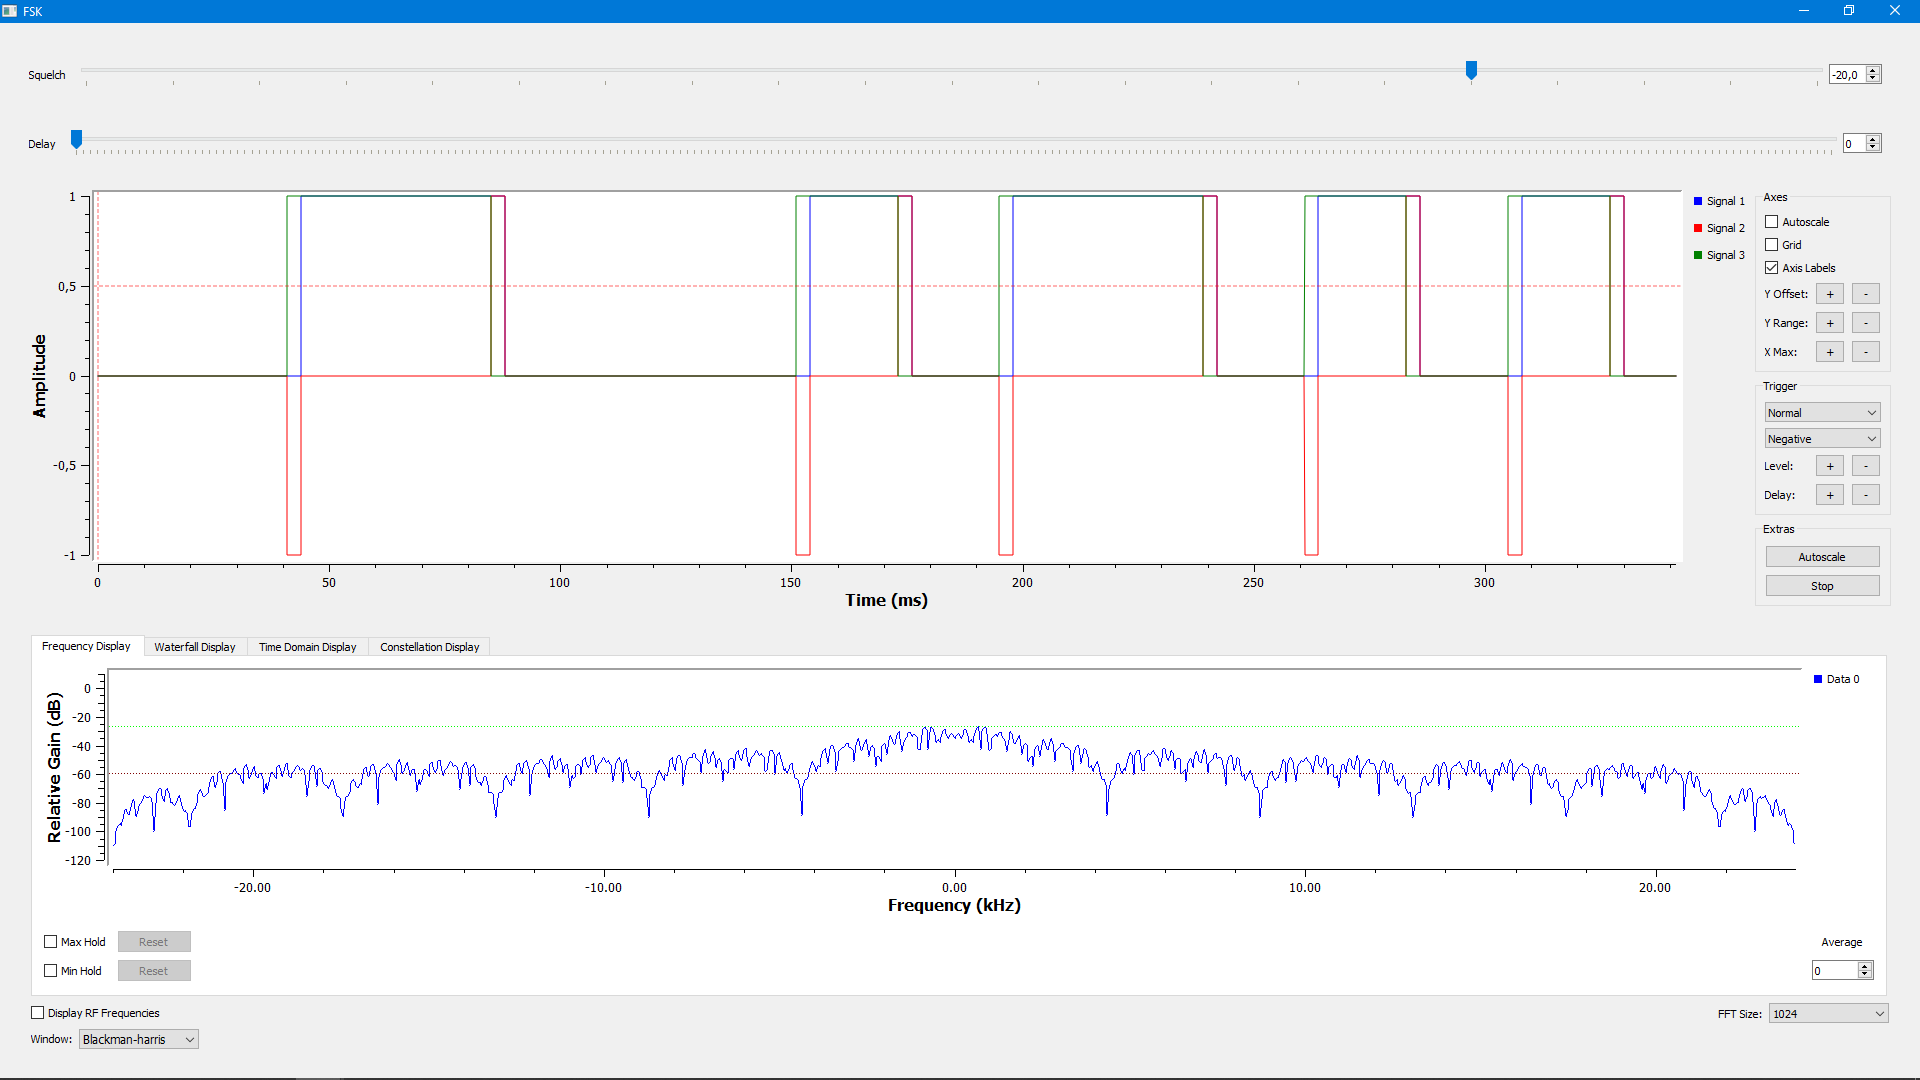
\includegraphics[scale=0.27]{fig/lab12/lab12_03.png}
		\caption{Тестирование без задержки с наложением шума}
		\label{pic:e1} % название для ссылок внутри кода
	\end{center}
\end{figure}

Исходя из Рисунка 12.3 видно, что у нас присутствует 3 сигнала. Синий сигнал - данные полученные приёмником. Зелёный сигнал - данные переданные передатчиком. Красный сигнал - разница между двумя предыдущими. Если всё передаётся верно, то красный сигнал должен быть равен 0. Исходя из результатов видно, что переднная и полученная информация разная. Дело в том, что всё блоки передатчика и приёмника не работают с бесконечно малой задержкой. Поэтому надо ввести задержку между приёмом и выдачей данных на диаграмму. Делается это при помощи блока Delay. Установил задержку 145.

    \begin{figure}[H]
	\begin{center}
		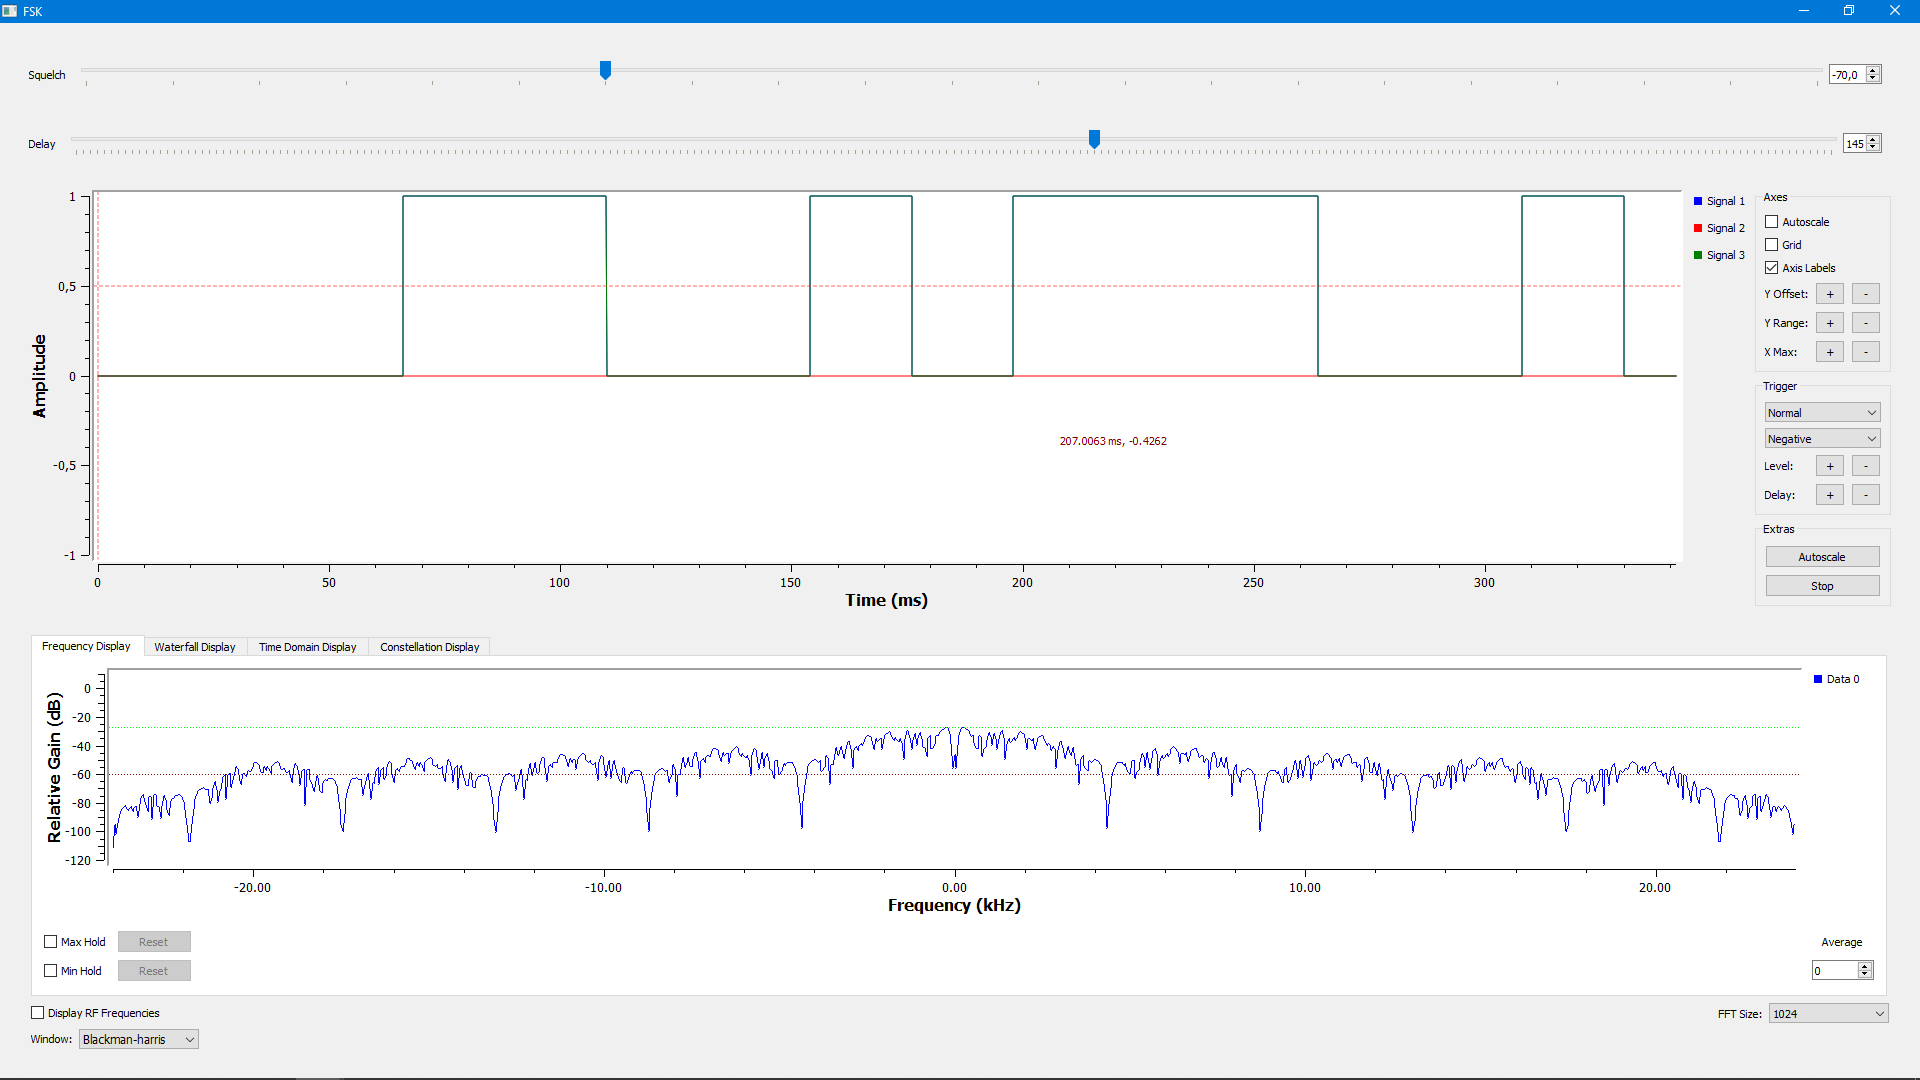
\includegraphics[scale=0.27]{fig/lab12/lab12_04.png}
		\caption{Тестирование с установленной задержкой}
		\label{pic:e1} % название для ссылок внутри кода
	\end{center}
\end{figure}

На рисунке видно, что мы подверги сигнал шумам, но из-за фильтра это не помешало нам получить информацию.

\subsection{Вывод}
В данной работе был изучен новый способ модуляции. Как говорилось ранее, он довольно шумоустойчив из-за того, что информация передаётся при помощи изменений частоты, а не амплитуды. При помощи среды Radio GNU была создана модель и проверена на корректность.